\subsection{Questionnaire}
\subsubsection{System Usefulness}

A strong and significant main effect of the interaction device was found on the \textsc{system usefulness} $(Z(1) = -3.517, p = .000437, r = .622)$.. The medians for the keyboard and leap modes were 6.8125 and 1.8125 respectively. See figure~\ref{fig:system_usefulness}.

\begin{figure}[H]
\centering
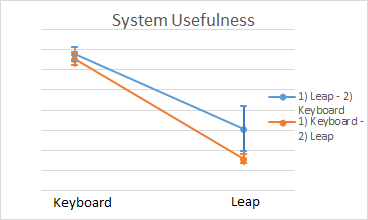
\includegraphics[width=0.5\textwidth]{imgs/results/system_usefulness}
\caption{System Usefulness - the mean and the 95\% intervals are plotted for both modes. The plots was split on the order of the interaction device. There is only a main effect of interaction device and no interaction device x order interaction effect.}
\label{fig:system_usefulness}
\end{figure}

\subsubsection{Interface Quality}

A strong and significant main effect of the interaction device was found on the \textsc{interface quality} $(Z(1) = -3.417, p = .000632, r = .604)$. The medians for the keyboard and leap modes were 6.167 and 3.833 respectively. See figure~\ref{fig:interface_quality}.

\begin{figure}[H]
\centering
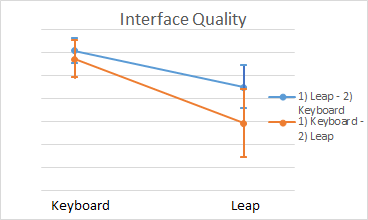
\includegraphics[width=0.5\textwidth]{imgs/results/interface_quality}
\caption{Interface Quality - the mean and the 95\% intervals are plotted for both modes. The plots was split on the order of the interaction device. There is only a main effect of interaction device and no interaction device x order interaction effect.}
\label{fig:interface_quality}
\end{figure}

\subsubsection{Qualitative responses}
\textbf{Easy to use}\newline
Question 1 and 2 in the after-trial questionnaire (see the appendix) were items that asked how easy to use the system was. For the LEAP-motion 16 out of 32 responses were recorded. 12.5\% of the users reported that it was impossible to grab a block that was already placed on the grid. 25\% users reported the bad registration and classification of the hand as troublesome. 19\% reported that grabbing in general was very difficult and 6\% reported that it was physically very tiring. 30\% viewed the concept of the system as very simple but managing it very hard.

For the keyboard and mouse 8 out 32 of responses were collected. 60\% perceived the system as very easy to use. 25\% commented on how intuitive the system was and 12.5\% made a comment on how counter intuitive the mouse wheel was. \newline

\noindent\textbf{Completing the tast}\newline
Question 3, 4 \& 5 in the after-trial questionnaire (see the appendix) were on how effectivly, fast and efficiently the user could complete the task. For the LEAP-motion 8 of the 48 open questions were answered. 50\% said completing the task took more effort than it needed to. Furthermore the remaining remarks were about the misconception of the system, unintended behavior by the system and slow response of the system as reasons why completing the task was not that efficient, effective or fast.

For the keyboard and mouse 6 out of 48 responses were collected. All but one respondent found the system very effective, efficient and fast. One made a remark that it started slow but that user also reported not really reading the instructions. \newline

\noindent\textbf{Easy to learn}\newline
Question 6,7 \& 8 in the after-trial questionnaire (see the appendix) were related to how easy to learn the system was. For the LEAP-motion 16 out of 48 responses were collected. 25\% thought the system as tiring and not comfortable, 25\% thought if they practiced more they could get better results and 25\% would like to wait for improvements in the system first. The rest of the responses made remarks that they did not understood the technology or were very new to this kind of devices.  

For the keyboard and mouse 3 out of 48 questions were filled in. All respondents reported that they knew how to operate the system so no learning was needed. \newline

\noindent\textbf{Interface Quality}\newline
Question 9,10 \& 11 in the after-trial questionnaire (see the appendix) were related to the interface and its functionalities. For the LEAP-motion 14 out of 48 questions were filled in. 60\% agreed that the LEAP-motion had a lot of potential that was not used in the experiment. 15\% did not used all the possible functions such as swipe. One respondent reported that prior experiences with the LEAP-motion did not match the experience during the experiment. A different user reported a desire for more feedback about the status of the system. 

For the keyboard and mouse 10 out of 48 responses were gathered. 40\% precieved the interface as adequate, 10\% thought it was great and another 10\% thought the LEAP-motion was more fun. 30\% had pointers to improve the functionality e.g. rotating the screen by dragging with the mouse or deleting a block by right clicking.\newline

\noindent\textbf{Overall remarks}\newline
In this paragraph the responses to question 12 in the after-trial questionnaire (see the appendix) and the items in the additional questionnaire are summarized. Most participants reported the experiment to be fun but difficult in the LEAP-motion conditions. Most participants would use the mouse and keyboard in every situation especially when they have to pick between the LEAP-motion and the keyboard + mouse. Most participants don’t know when they want to use the LEAP-motion and the ones that do report that they would use it for games. \newline


